\documentclass[journal]{IEEEtran}
\usepackage[utf8]{inputenc}
%\usepackage{minted}
\usepackage{booktabs}
\usepackage{color}
\usepackage{commath}
\usepackage{tikz}
\usepackage[official]{eurosym}
\usepackage{fontawesome}
\usepackage{breqn}
\usepackage{float}
\usepackage{mathtools}
\usepackage{amsthm}

\usepackage{mathrsfs}

\newtheorem{theorem}{Theorem}

\usepackage[binary-units=true]{siunitx}

%\newcommand{\py}[1]{\mintinline{python}{#1}}

\title{Artificial Intelligence (\texttt{LINGI2261}) \\ Assignment 2 --- Group 13}
\author{Martin Braquet, Gilles Peiffer}

\begin{document}

\maketitle

\section{A* Versus Uniform-Cost Search}

\subsection{A Consistent and Admissible Heuristic}

A valid heuristic for this problem is the Manhattan distance between the two symbols' positions, which is the minimum distance between them expressed in number of tiles.

\begin{theorem}[Consistency of Manhattan distance heuristic]
	\label{thm:cons}
	The Manhattan distance is a consistent heuristic for the unweighted grid search problem.
\end{theorem}
\begin{proof}
It is consistent for an unweighted grid since at each move, where the traveller can at most decrease the remaining cost to the goal by one, the heuristic is also decreased by one.
Formally, for every node $N$ and each successor $P$ of $N$, consistency states that the estimated cost of reaching the goal from $N$ is no greater than the step cost of getting to $P$ plus the estimated cost of reaching the goal from $P$:
\[
 h(N) \le c(N,P) + h(P).
\]
In our case, let us define $N = (x_N, y_N)$ by its coordinates on the 2D grid.
In the same way, we define $P = (x_P, y_P)$ and the goal $G = (x_G, y_G)$. The inequality can thus be rewritten as
\[
 \abs{x_N - x_G} + \abs{y_N - y_G} \le 1 + \abs{x_P - x_G} + \abs{y_P - y_G},
\]
where $c(N,P) = 1$ since $P$ is the successor of $N$ and the grid is unweighted.
Using the triangle inequality, one can rewrite $\abs{x_N - x_G} + \abs{y_N - y_G}$ as 
\begin{align*}
   & \abs{x_N - x_P + x_P - x_G} + \abs{y_N - x_P + x_P - y_G} \\
  {}\le{}& \abs{x_N - x_P} + \abs{x_P - x_G} + \abs{y_N - x_P} + \abs{x_P - y_G} \\
  {}\le{}& 1 + \abs{x_P - x_G} + \abs{x_P - y_G},
\end{align*}
since $\abs{x_N - x_P} + \abs{x_N - y_P} = 1$ since the traveller moves by one tile either horizontally or vertically.
It has thus been proven that this heuristic is consistent.
\end{proof}
\begin{theorem}[Admissibility of Manhattan distance heuristic]
	\label{thm:admiss}
	The Manhattan distance is an admissible heuristic for the weighted grid search problem.
\end{theorem}
\begin{proof}
If a heuristic is consistent, it is also admissible.
The Manhattan distance is thus also always lower than or equal to the real number of moves to the goal.
Formally, $h(h)$ is admissible if, for all nodes $n$, $h(n) \le C^*$, where $C^*$ is the lowest path cost among all solutions.
Since each action can move only one tile, performing an action can at most reduce $h$ by one.
Since the goal can be reached in $C^*$ actions, we thus have $h(n) - C^* \le h(G) = 0$. Therefore, we have $h(n) \le C^*$ for all $n$, and $h$ is admissible.
\end{proof}

\subsection{Uniform-Cost Graph Search}

The visited nodes (in light gray) for the uniform-cost graph search are depicted in Figure~\ref{fig:maze1}, the number in each tile decribes the order of the visited states.
The uniform-cost search finds the solution when it reaches the 25th state.

\begin{figure}[H]
 \centering
 \resizebox{0.34\textwidth}{!}{
 \begin{tikzpicture}
    [
        box/.style={rectangle,draw=black,thick, minimum size=1cm},
    ]

    \foreach \x in {1,...,7}{
        \foreach \y in {1,...,7}
            \node[box] at (\x,\y){};
    }
	\foreach \x in {0,...,6}{
		\node at (0, \x+1){\scriptsize \x};
		\node at (\x+1,0){\scriptsize \x};
	}
	
	\node at (-1, 4){\(j\)};
	\node at (4, -1){\(i\)};


    \node[box,fill=black] at (6,7){};
    \node[box,fill=black] at (6,6){};
    \node[box,fill=black] at (5,6){};
    \node[box,fill=black] at (4,5){};
    \node[box,fill=black] at (3,5){};
    \node[box,fill=black] at (2,5){};
    \node[box,fill=black] at (3,4){};
    \node[box,fill=black] at (3,3){};
    \node[box,fill=black] at (3,2){};
    \node[box,fill=black] at (2,2){};
    \node[box,fill=black] at (7,4){};
    \node[box,fill=black] at (7,3){};
    \node[box,fill=black] at (7,2){};
    
    \node[box,fill=lightgray] at (5,7){};
    \node[box,fill=lightgray] at (4,7){1};
    \node[box,fill=lightgray] at (3,7){2};
    \node[box,fill=lightgray] at (4,6){3};
    \node[box,fill=lightgray] at (2,7){4};
    \node[box,fill=lightgray] at (3,6){5};
    \node[box,fill=lightgray] at (1,7){6};
    \node[box,fill=lightgray] at (2,6){7};
    \node[box,fill=lightgray] at (1,6){8};
    \node[box,fill=lightgray] at (1,5){9};
    \node[box,fill=lightgray] at (1,4){10};
    \node[box,fill=lightgray] at (1,3){11};
    \node[box,fill=lightgray] at (2,4){12};
    \node[box,fill=lightgray] at (1,2){13};
    \node[box,fill=lightgray] at (2,3){14};
    \node[box,fill=lightgray] at (1,1){15};
    \node[box,fill=lightgray] at (2,1){16};
    \node[box,fill=lightgray] at (3,1){17};
    \node[box,fill=lightgray] at (4,1){18};
    \node[box,fill=lightgray] at (4,2){19};
    \node[box,fill=lightgray] at (5,1){20};
    \node[box,fill=lightgray] at (4,3){21};
    \node[box,fill=lightgray] at (5,2){22};
    \node[box,fill=lightgray] at (6,1){23};
    \node[box,fill=lightgray] at (4,4){};
    
    \node[box] at (5,7){\faMale};
    \node[box] at (4,4){\euro{}};

 \end{tikzpicture}}
 \caption{Visited nodes (in light gray) for the uniform-cost graph search.}
 \label{fig:maze1}
\end{figure}

\subsection{A* Graph Search}

The visited nodes (in light gray) for the A* graph search are depicted in Figure~\ref{fig:maze2}.
A* finds the solution when it reaches the 22nd state.

\begin{figure}[H]
 \centering
 \resizebox{0.34\textwidth}{!}{
 \begin{tikzpicture}
    [
        box/.style={rectangle,draw=black,thick, minimum size=1cm},
    ]

    \foreach \x in {1,...,7}{
        \foreach \y in {1,...,7}
            \node[box] at (\x,\y){};
    }
    \foreach \x in {0,...,6}{
        \node at (0, \x+1){\scriptsize \x};
        \node at (\x+1,0){\scriptsize \x};
    }

    \node at (-1, 4){\(j\)};
    \node at (4, -1){\(i\)};

    \node[box,fill=black] at (6,7){};
    \node[box,fill=black] at (6,6){};
    \node[box,fill=black] at (5,6){};
    \node[box,fill=black] at (4,5){};
    \node[box,fill=black] at (3,5){};
    \node[box,fill=black] at (2,5){};
    \node[box,fill=black] at (3,4){};
    \node[box,fill=black] at (3,3){};
    \node[box,fill=black] at (3,2){};
    \node[box,fill=black] at (2,2){};
    \node[box,fill=black] at (7,4){};
    \node[box,fill=black] at (7,3){};
    \node[box,fill=black] at (7,2){};
    
    \node[box,fill=lightgray] at (5,7){};
    \node[box,fill=lightgray] at (4,7){1};
    \node[box,fill=lightgray] at (3,7){4};
    \node[box,fill=lightgray] at (4,6){2};
    \node[box,fill=lightgray] at (2,7){6};
    \node[box,fill=lightgray] at (3,6){3};
    \node[box,fill=lightgray] at (1,7){10};
    \node[box,fill=lightgray] at (2,6){5};
    \node[box,fill=lightgray] at (1,6){7};
    \node[box,fill=lightgray] at (1,5){8};
    \node[box,fill=lightgray] at (1,4){9};
    \node[box,fill=lightgray] at (1,3){12};
    \node[box,fill=lightgray] at (2,4){11};
    \node[box,fill=lightgray] at (1,2){14};
    \node[box,fill=lightgray] at (2,3){13};
    \node[box,fill=lightgray] at (1,1){15};
    \node[box,fill=lightgray] at (2,1){16};
    \node[box,fill=lightgray] at (3,1){17};
    \node[box,fill=lightgray] at (4,1){18};
    \node[box,fill=lightgray] at (4,2){19};
    \node[box,fill=lightgray] at (4,3){20};
    \node[box,fill=lightgray] at (4,4){};
    
    \node[box] at (5,7){\faMale};
    \node[box] at (4,4){\euro{}};

 \end{tikzpicture}}
 \caption{Visited nodes (in light gray) for the A* graph search search.}
 \label{fig:maze2}
\end{figure}

\section{Pacmen Problem}
\subsection{Model}
\subsubsection{States}
The states are described by a grid detailing the content of the different tiles: a wall or border tile, a Pacman, some food, or an empty tile.
%the content description of the maze. A \@ in a cell represents food, a \$ is a Pacman and a x is a wall. The other variables of the state are \py{nbr} (the number of rows), \py{nbc} (the number of columns), \py{pac_list} (the positions of the Pacmen) and \py{food_list} (the positions of the food).
\subsubsection{Initial States}
The initial state can be any state, provided that it has at least one tile filled with food, and one tile filled with a Pacman (and a border going around the grid).

\subsubsection{Transition Model}
A simple formulation defines the actions as a list of movements (Left, Right, Up, Down, Stay) for each Pacman on the board.
Two additional constraints exist: at least one Pacman must move (e.g. have an action which is not ``Stay'') at each turn, and a given Pacman can only make one move at each turn.
Different subsets of actions are possible depending on where the Pacmen are (e.g. blocked by the borders, the walls or each other). 
Given a state and action, the transition model returns the resulting state, that is, the same grid as before, except that the Pacmen which received an action command have been moved accordingly, possibly removing food on the tile where they arrived if there was any and filling up empty tiles otherwise.

\subsubsection{Goal Test}
The goal test checks whether there is no food on the board, which means that there is no cell in the grid filled with food.
A counter of remaining food cells is used in order to reduce the computation time of the goal test.

\subsubsection{Path Cost Function}
Since each step has unitary cost, the path cost function is the number of steps in the path: $g(n) = d_n$ where $d_n$ is the depth of the node $n$.


\subsection{Maximum Branching Factor}
Since each Pacman can move up to four positions or stay where it is, $k$ Pacmen can move to $5^k-1$ different states (since at least one Pacman has to move and the case where no Pacmen move is thus not possible).
The maximum branching factor is thus $5^k-1$.
This exponential branching factor can lead to complex trees if the number of Pacmen is very high.


\subsection{Admissible Heuristic For One Pacman}
%Sum of Manhattan distances between Pacman - nearest food - nearest food to previous food - ...
\subsubsection{Heuristic}
The heuristic for a single Pacman is as follows: for state $N$,
\[
 h(N) = \sum_{i=1}^n d(x_{i-1},x_i),
\]
where $d(A,B)$ is the Manhattan distance between the points $A$ and $B$, $x_0$ is the position of the Pacman and $x_i$ (for \(i = 1, \ldots, n\)) is the position (which has not yet been selected) of the food closest to $x_{i-1}$.
Formally, if \(\mathscr{F}_i\) is the set of  unvisited food tiles when looking for \(x_i\), then
\[
x_{i} = \min_{j \in \mathscr{F}_i} d(x_{i-1}, x_j), \quad \forall i = 1, \ldots, n.
\]

\subsubsection{Admissibility}
This heuristic is admissible since it uses the Manhattan distance, which is always less than or equal to the true distance, as shown in Theorem~\ref{thm:admiss}.

\subsubsection{Complexity}
As with any A* search algorithm, the complexity is exponential in the depth \(d\) of the shallowest goal state, where the base is the effective branching factor \(b^\varepsilon\) (where \(\varepsilon\) is the relative error of the heuristic).
This can be shown by observing that the number of explored nodes is \(\sum_{i=1}^d b^{\varepsilon i} \in \mathcal{O}(b^{\varepsilon d})\).

\subsection{Admissible Heuristic For \(k\) Pacmen}
\subsubsection{Heuristic}
The generalization for $k$ Pacmen is achieved by successively applying the procedure for one Pacman to all Pacmen.
A list of foods $\ell_{P_i}$ ($i=1,\dots,k$) is associated to each Pacman.
The first element of the list is the position of the Pacman.
We also create a list of all food tiles on the board, \(\mathscr{L}\), which we use for bookkeeping later on.

For each Pacman $P_i$, one can then remove the closest food tile $f_j$ ($j=1,\dots,n$) from the list of foods \(\mathscr{L}\), and add this food to the list $\ell_{P_i}$ of the related Pacman.
The closest food tile $f_j$ is computed by using the Manhattan distance between the food tile $f_j$ and the most recent element of the list $\ell_{P_i}$.

Applying this procedure allows to create a successive list of targets for each Pacman; the heuristic \(h_i\) for Pacman $P_i$ is thus the sum of the Manhattan distances between each element in its list $\ell_{P_i}$.

Finally, the solution will be found when each Pacman has achieved its path given by its associated list.
Thus, the heuristic is given by the maximum path cost of the Pacmen:
\begin{align*}
 h(n) &= \max_{i = 1,\ldots,k} h_i(n) \\
 &= \max_{i=1,\ldots, k} \left(\sum_{\alpha=1}^{\mathrm{length}(\ell_{P_i})} d\left(\ell_{P_i}[\alpha],\ell_{P_i}[\alpha-1]\right)\right).
\end{align*}

\subsubsection{Admissibility}
Since all individual heuristics \(h_i\) are admissible (by the same argument as above), one can deduce that their maximum must also be admissible.

\subsubsection{Complexity}
By the same reasoning as before, the complexity is exponential, in \(\mathcal{O}(b^{\varepsilon d})\), where \(d\) is the depth of the shallowest goal state, \(\varepsilon\) is the relative error of the heuristic and \(b^\varepsilon\) is the effective branching factor.

\subsection{Implementation}
The program is uploaded on INGInious.

\subsection{Experiment}
\begin{table}[!hbtp]
	\centering
	\begin{tabular}{c@{\hspace{0.7cm}}ccc|ccc} 
		\toprule
		Inst. & \multicolumn{3}{c}{A*} & \multicolumn{3}{c}{BFS} \\
		\midrule
		1 & 0.974 & 9 & 16  & 1.32 & 9 & 63 \\
		2 & 3.10 & 19 & 53 & 80.6 & 19 & 984 \\
		3 & 6.10 & 25 & 119 & 4.29 & 25 & 168 \\
		4 & 3.78 & 13 & 71 & 3.41 & 13 & 126 \\
		5 & 2.81 & 13 & 53 & 2.50 & 13 & 81 \\
		6 & 5.16 & 25 & 101 & 3.77 & 25 & 157 \\
		7 & 14.3 & 25 & 175 & 11.8 & 25 & 238 \\
		8 & 23.0 & 33 & 348 & 18.5 & 33 & 466 \\
		9 & 69.6 & 13 & 791  & 96.4 & 13 & 2865 \\
		10 & 161 & 8 & 1329 & 1880 & 8 & 40282 \\
		\bottomrule \\
	\end{tabular}
	\caption{Comparison of execution times for various algorithms.
		The first column contains the execution times, given with 3 significant figures in milliseconds; the second contains the number of moves in the solution and the third contains the number of explored nodes.}
	\label{time1}
\end{table}

 The computation times for the two algorithms on each of the 10 instances are detailed in Table~\ref{time1}.\footnote{Experiments were run on an Early 2015 MacBook Pro, running macOS Sierra 10.12.6, using a \SI{2.9}{\giga\hertz} Intel Core i5 processor, with \SI{8}{\giga\byte} of \SI{1867}{\mega\hertz} DDR3 RAM and an Intel Iris Graphics 6100 GPU.} 

As we can see, the number of nodes explored using A* search is lower than the number of nodes explored with breadth-first search for all ten instances.

Computation times are not always strictly lower for A* search, though the difference is quite small (instances 3, 4, 6, 7 and 8 took slightly longer for A* search than for BFS).

The reason for this is that our heuristic is quite complicated to compute, and in cases where BFS finds a solution relatively quickly, the heuristic does not improve the number of explored nodes by much (but does require a lot more computation effort).
The reason why A* consistently explores less nodes is because BFS can simply be seen as A* with a constant heuristic, which is not as good as the heuristic we use.

\subsection{Program submission}
The program is uploaded on INGInious.

\end{document}
